% !TEX program = pdflatex
\documentclass[10pt,twocolumn,a4paper]{article}

% ── packages ──
\usepackage[utf8]{inputenc}
\usepackage[T1]{fontenc}
\usepackage{lmodern}
\usepackage[margin=1.8cm]{geometry}
\usepackage{graphicx}
\usepackage{amsmath,amssymb}
\usepackage{booktabs}
\usepackage{enumitem}
\usepackage{xcolor}
\usepackage{listings}
\usepackage{float}
\usepackage{caption}
\usepackage{hyperref}
\usepackage{titlesec}

\hypersetup{colorlinks=true,linkcolor=blue!60!black,citecolor=blue!60!black,urlcolor=blue!60!black}

\titlespacing*{\section}{0pt}{1.2ex plus .2ex minus .1ex}{0.6ex plus .1ex}
\titlespacing*{\subsection}{0pt}{0.8ex plus .2ex minus .1ex}{0.4ex plus .1ex}

\setlength{\parskip}{0.4em}
\setlength{\parindent}{0em}

\lstset{
  basicstyle=\ttfamily\scriptsize,
  frame=single,
  breaklines=true,
  columns=fullflexible,
}

% ══════════════════════════════════════════════════════════════
\begin{document}

% ── Title ──
\twocolumn[{%
\begin{center}
  {\LARGE\bfseries Song Song --- Parallel P2P Download Infrastructure}\\[0.6em]
  {\large Master 1 $\cdot$ System Architecture $\cdot$ USTH $\cdot$ 2025--2026}\\[0.8em]
  \begin{tabular}{ccl}
    \toprule
    \textbf{Student ID} & \textbf{Name} & \textbf{Email} \\
    \midrule
    2540008 & Nguy\~{e}n Phong Ch\^{a}u & chaunp.2540008@usth.edu.vn \\
    2540023 & L\^{e} Nghi\^{e}m Thanh Th\d{u}y & thuylnt.2540023@usth.edu.vn \\
    \bottomrule
  \end{tabular}
\end{center}
\vspace{1em}
}]

% ══════════════════════════════════════════════════════════════
\section*{Abstract}

Song Song is a pure-Java P2P file-download system: a central Directory (RMI) tracks live Daemon peers; a Download client fragments the target file and drains a shared work-stealing queue in parallel across $N$ Daemon threads. This report covers the basic prototype, an empirical parallelism validation on AWS EC2, and three system enhancements.

% ══════════════════════════════════════════════════════════════
\section{Architecture}

The system follows a \textbf{three-tier architecture} inspired by the BitTorrent model, implemented entirely in Java without any third-party networking library.

{\scriptsize
\begin{verbatim}
    +-------------------------+
    |  Directory (RMI :1099)  |
    |  . file->Daemon registry|
    |  . load counters        |
    |  . heartbeat/sweep      |
    +---+-----------------+---+
        |                 |
    RMI:register    RMI:getSources
    /heartbeat      (sorted by load)
        |                 |
   +----+----+            |
   |         |            |
+--v---+ +---v--+         |
|Dmn A | |Dmn B |         |
|:6000 | |:6001 |         | 
+--+---+ +--+---+         | 
   |  TCP:   |      +-----v-------+
   | GET_SIZE      .| Download    |
   |  /GET_FRAGMENT | N workers   |
   +---------+----> | shared queue|
                    +-------------+
\end{verbatim}     
}

\begin{table}[H]
\centering
\caption{Communication channels}
\scriptsize
\begin{tabular}{@{}lll@{}}
\toprule
\textbf{Channel} & \textbf{Protocol} & \textbf{Calls} \\
\midrule
Daemon $\to$ Dir. & Java RMI & \texttt{register}, \texttt{unregister}, \\
 & & \texttt{heartbeat}, $\pm$\texttt{load} \\
Download $\to$ Dir. & Java RMI & \texttt{getSourcesForFile} \\
Download $\to$ Daemon & Raw TCP & \texttt{GET\_SIZE}, \texttt{GET\_FRAG.} \\
\bottomrule
\end{tabular}
\end{table}

The Directory is backed by two \texttt{ConcurrentHashMap}s: \texttt{fileToClients} (filename $\to$ set of Daemon IDs) and \texttt{clients} (Daemon ID $\to$ \texttt{ClientInfo}). Mutations are \texttt{synchronized} to prevent races under concurrent registrations and sweeps.

% ══════════════════════════════════════════════════════════════
\section{Enhancements}

\textbf{2.1 Failure handling \& retry.}
If a fragment transfer fails, the fragment index is returned to the shared queue and the worker exits --- other workers pick up the orphaned fragment. Each fragment is retried up to a fixed limit before being marked permanently failed. After all wave-1 workers complete, any remaining fragments trigger a \textbf{second wave}: the client re-fetches the source list from the Directory and launches a fresh set of workers. This covers both transient network errors and Daemons that crashed partway through a transfer.

\textbf{2.2 Dynamic adaptation.}
\begin{itemize}[nosep,leftmargin=1.5em]
  \item \textit{Heartbeat \& auto re-registration:} Daemons heartbeat every \textbf{5\,s} (delta file list only when changed); the Directory sweeper evicts clients silent for $>$\textbf{15\,s}. \texttt{Ctrl+C} calls \texttt{unregister()} via a JVM shutdown hook. If a Daemon is evicted and then heartbeats, \texttt{heartbeat()} returns \texttt{false} and the Daemon silently re-registers. Newly downloaded files are announced on the next heartbeat, making the downloader an instant source.
  \item \textit{Load-aware source selection:} The Directory increments a per-Daemon \texttt{load} counter on \texttt{GET\_FRAGMENT} and decrements on completion; \texttt{getSourcesForFile} returns sources sorted by load ascending. Sources with \texttt{load > 10} are dropped unless doing so would leave zero sources.
\end{itemize}

\textbf{2.3 Conditional GZIP compression.}
The Daemon compresses each fragment and sends the compressed payload only if it is smaller than the raw data; otherwise raw bytes are sent with \texttt{compressed=false}. Transparent decompression is done client-side. Effective for text/sparse-binary files; zero overhead for pre-compressed formats (MP4, ZIP, JPEG).

% ══════════════════════════════════════════════════════════════
\section{How to Run}

\subsection{Prerequisites}
Java 17 (JDK), Linux (tested on Ubuntu/WSL).

\subsection{Compile}
\begin{lstlisting}
cd /path/to/sujet_project
bash compile.sh
\end{lstlisting}

\subsection{Step 1 --- Start Directory}
\begin{lstlisting}
./run_directory.sh [rmiPort] [myHost]
\end{lstlisting}

\begin{table}[H]
\centering\scriptsize
\begin{tabular}{@{}lll@{}}
\toprule
\textbf{Parameter} & \textbf{Default} & \textbf{Description} \\
\midrule
rmiPort & 1099 & RMI registry port \\
myHost  & auto & IP of this machine \\
\bottomrule
\end{tabular}
\end{table}

Example:
\begin{lstlisting}
./run_directory.sh
./run_directory.sh 1099 172.20.242.201
\end{lstlisting}

\subsection{Step 2 --- Start Daemon(s)}
\begin{lstlisting}
./run_daemon.sh [dirHost] [dirPort]
  [sharedFolder] [myHost] [daemonPort]
\end{lstlisting}

\begin{table}[H]
\centering\scriptsize
\begin{tabular}{@{}lll@{}}
\toprule
\textbf{Parameter} & \textbf{Default} & \textbf{Description} \\
\midrule
dirHost      & localhost & IP of Directory machine \\
dirPort      & 1099      & RMI port of Directory \\
sharedFolder & ./shared  & Folder with files to share \\
myHost       & auto      & IP of this machine \\
daemonPort   & 6000      & TCP port for fragments \\
\bottomrule
\end{tabular}
\end{table}

Examples:
\begin{lstlisting}
# Single machine test
./run_daemon.sh localhost 1099 ./shared1 \
  localhost 6000

# Cross-machine
./run_daemon.sh 172.20.242.201 1099 \
  ./shared1 192.168.1.10 6000
\end{lstlisting}

\subsection{Step 3 --- Download a File}
\begin{lstlisting}
./run_download.sh <filename> [dirHost]
  [dirPort] [outputFolder] [myHost]
  [compress] [fragmentKB]
\end{lstlisting}

\begin{table}[H]
\centering\scriptsize
\begin{tabular}{@{}lll@{}}
\toprule
\textbf{Parameter} & \textbf{Default} & \textbf{Description} \\
\midrule
filename     & \textit{required} & Name of file to download \\
dirHost      & localhost & IP of Directory machine \\
dirPort      & 1099      & RMI port of Directory \\
outputFolder & ./shared  & Output directory \\
myHost       & auto      & IP of this machine \\
compress     & false     & Enable GZIP (true/false) \\
fragmentKB   & 512       & Fragment size in KB \\
\bottomrule
\end{tabular}
\end{table}

Examples:
\begin{lstlisting}
# Basic download
./run_download.sh movie.mp4 172.20.242.201 \
  1099 ./output 172.20.242.201

# With compression and 256KB fragments
./run_download.sh movie.mp4 172.20.242.201 \
  1099 ./output 172.20.242.201 true 256
\end{lstlisting}

\subsection{Shutdown}
Press \texttt{Ctrl+C} to stop any component. Recommended order: \textbf{Download $\to$ Daemon $\to$ Directory}.

\begin{itemize}[nosep,leftmargin=1.5em]
  \item \texttt{Ctrl+C} on Daemon: triggers shutdown hook $\to$ calls \texttt{unregister()} $\to$ Directory removes it immediately
  \item If Daemon crashes without \texttt{Ctrl+C}: Directory detects via heartbeat timeout after 15\,s
\end{itemize}

% ══════════════════════════════════════════════════════════════
\section{Parallelism Validation}

\subsection{Experimental Setup}

\begin{itemize}[nosep,leftmargin=1.5em]
  \item 8 heterogeneous EC2 Daemons (multi-region)
  \item 1 Directory, 2 clients
  \item Variables: Sources 1--9, Fragment size 128\,KB--2\,MB, Compression ON/OFF
\end{itemize}

System behavior follows three regimes:
\begin{itemize}[nosep,leftmargin=1.5em]
  \item \textbf{Small files ($<$10\,MB)} $\to$ overhead dominated
  \item \textbf{Medium files ($\sim$50\,MB)} $\to$ parallelism dominated
  \item \textbf{Large files ($>$100\,MB)} $\to$ bandwidth + tail latency dominated
\end{itemize}

% ── Results ──
\subsection{Results}

\subsubsection{Fig.\ 1 --- Small file: test-medium.bin (5\,MB)}

\begin{figure}[htbp]
\centering
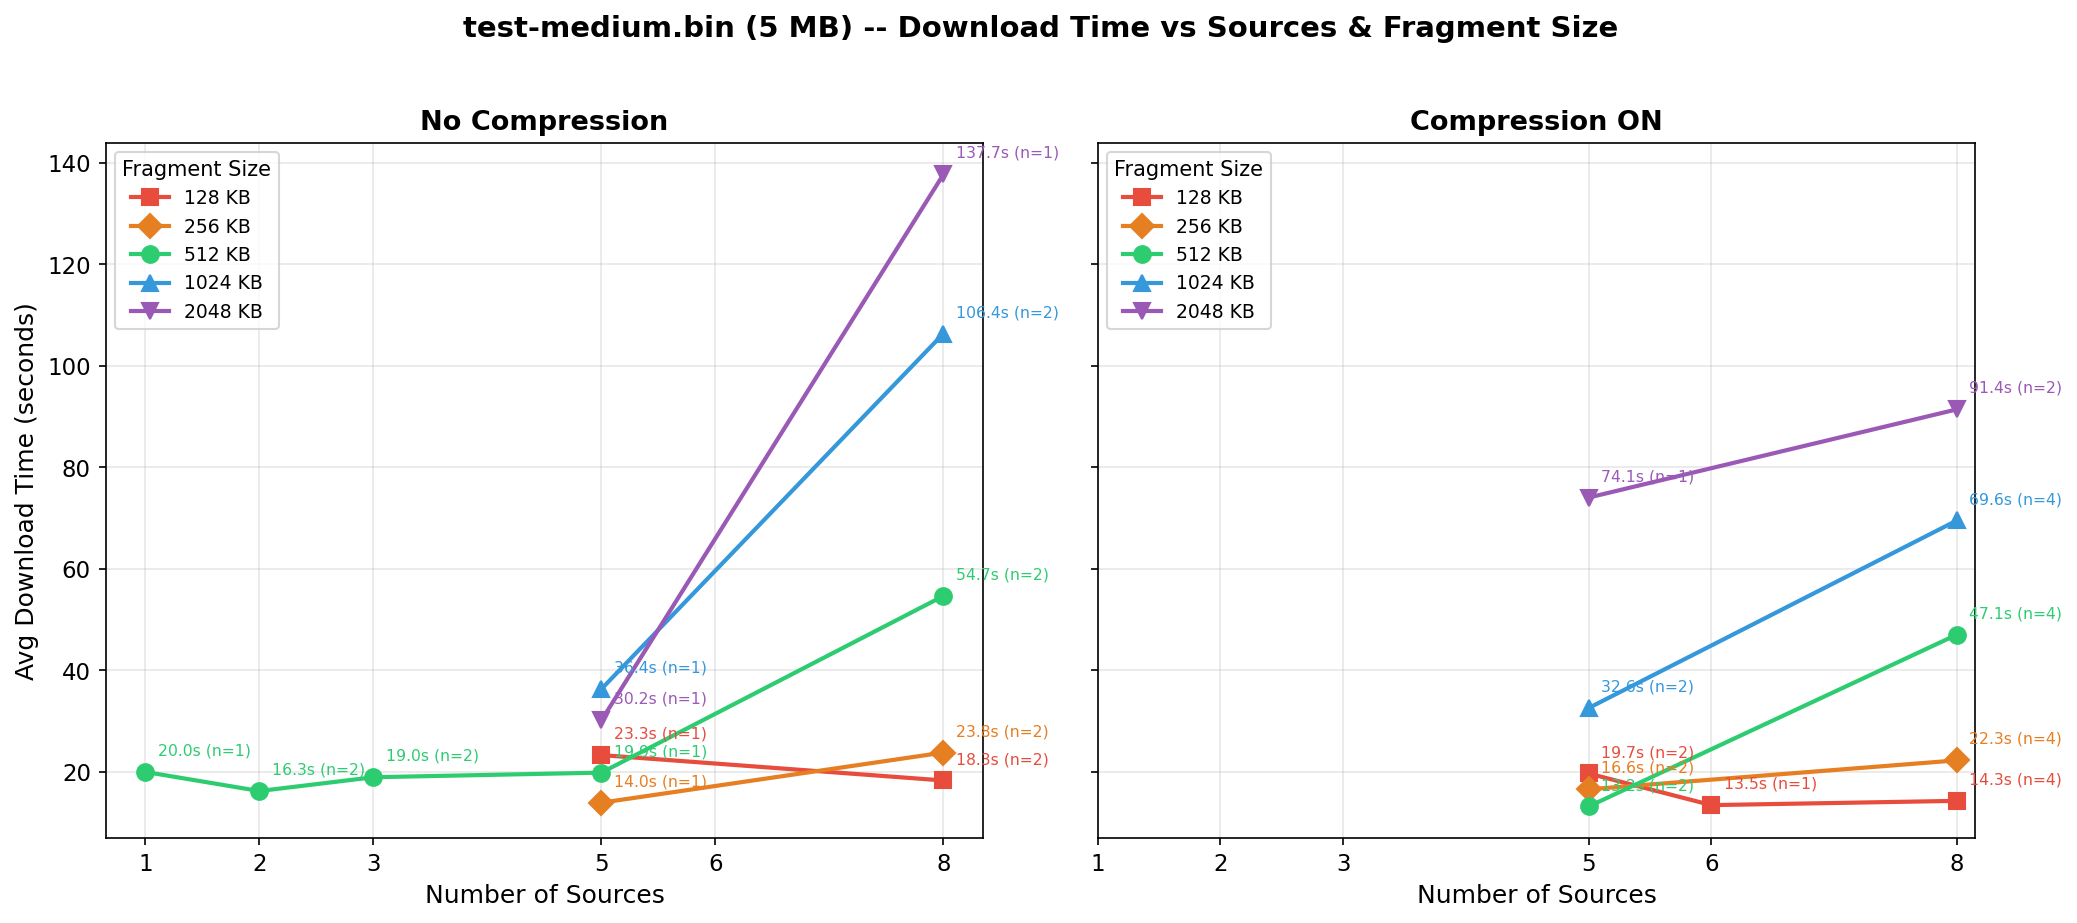
\includegraphics[width=\columnwidth,keepaspectratio,height=0.28\textheight]{image.png}
\caption{test-medium.bin (5\,MB) --- Download time vs.\ sources \& fragment size.}
\label{fig:medium}
\end{figure}

\begin{itemize}[nosep,leftmargin=1.5em]
  \item \textbf{128--256\,KB}: stable $\sim$12--24\,s regardless of source count --- fine granularity prevents any single slow source from becoming a bottleneck.
  \item \textbf{512\,KB}: good with 1--3 sources ($\sim$16--20\,s), but degrades to $\sim$54\,s at 8 sources.
  \item \textbf{1--2\,MB + 8 sources}: catastrophic (104--138\,s) --- only 3--5 fragments in the queue; the slowest source (10\,KB/s) must carry an entire megabyte fragment.
  \item Compression partially rescues large fragments (8 sources, 1024\,KB: 106$\to$69\,s) but cannot offset the root cause.
\end{itemize}

\textbf{Conclusion.} For $\sim$5\,MB files: \textbf{2--3 sources + 512\,KB fragment} or \textbf{many sources + 128--256\,KB fragment}. Compression unnecessary.

% ──────────────────────────────────────────────
\subsubsection{Fig.\ 2 --- Small file: Acclaim \& Response (9.5\,MB)}

\begin{figure}[htbp]
\centering
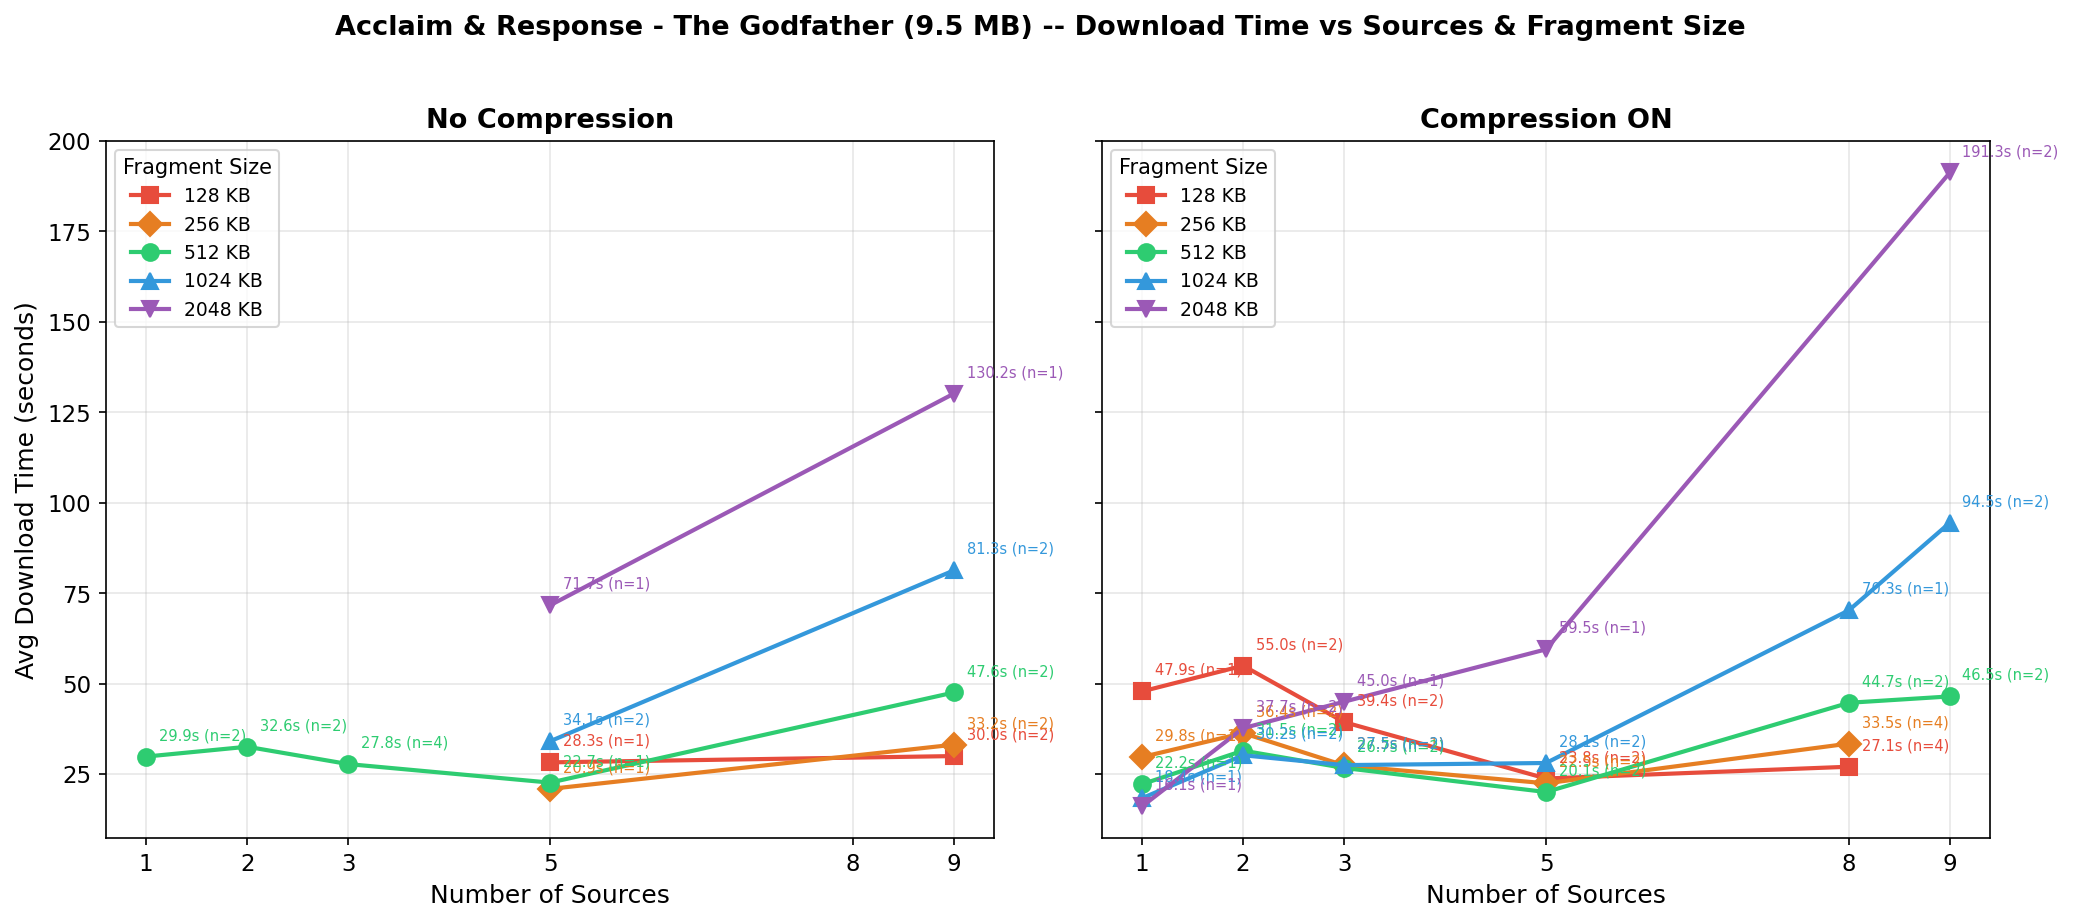
\includegraphics[width=\columnwidth,keepaspectratio,height=0.28\textheight]{image-1.png}
\caption{Acclaim \& Response (9.5\,MB) --- Download time vs.\ sources \& fragment size.}
\label{fig:acclaim}
\end{figure}

\begin{itemize}[nosep,leftmargin=1.5em]
  \item \textbf{512\,KB \& 1024\,KB}: stable $\sim$28--47\,s across 1--9 sources --- the sweet spot for this file size.
  \item \textbf{2048\,KB + 9 sources}: collapses to $\sim$130\,s --- only 5 fragments total; slowest worker determines finish time.
  \item \textbf{128\,KB compressed + 9 sources}: surges to $\sim$130\,s --- 76 fragments across 9 threads generates excessive scheduling overhead.
  \item Adding sources beyond 2--3 yields no benefit; the queue is too small to keep extra workers busy.
\end{itemize}

\textbf{Conclusion.} For $\sim$10\,MB files: \textbf{2--3 sources + 512\,KB fragment} ($\sim$28\,s). Adding more sources does not help.

% ──────────────────────────────────────────────
\subsubsection{Fig.\ 3 --- Medium file: test-large.bin (50\,MB)}

\begin{figure}[htbp]
\centering
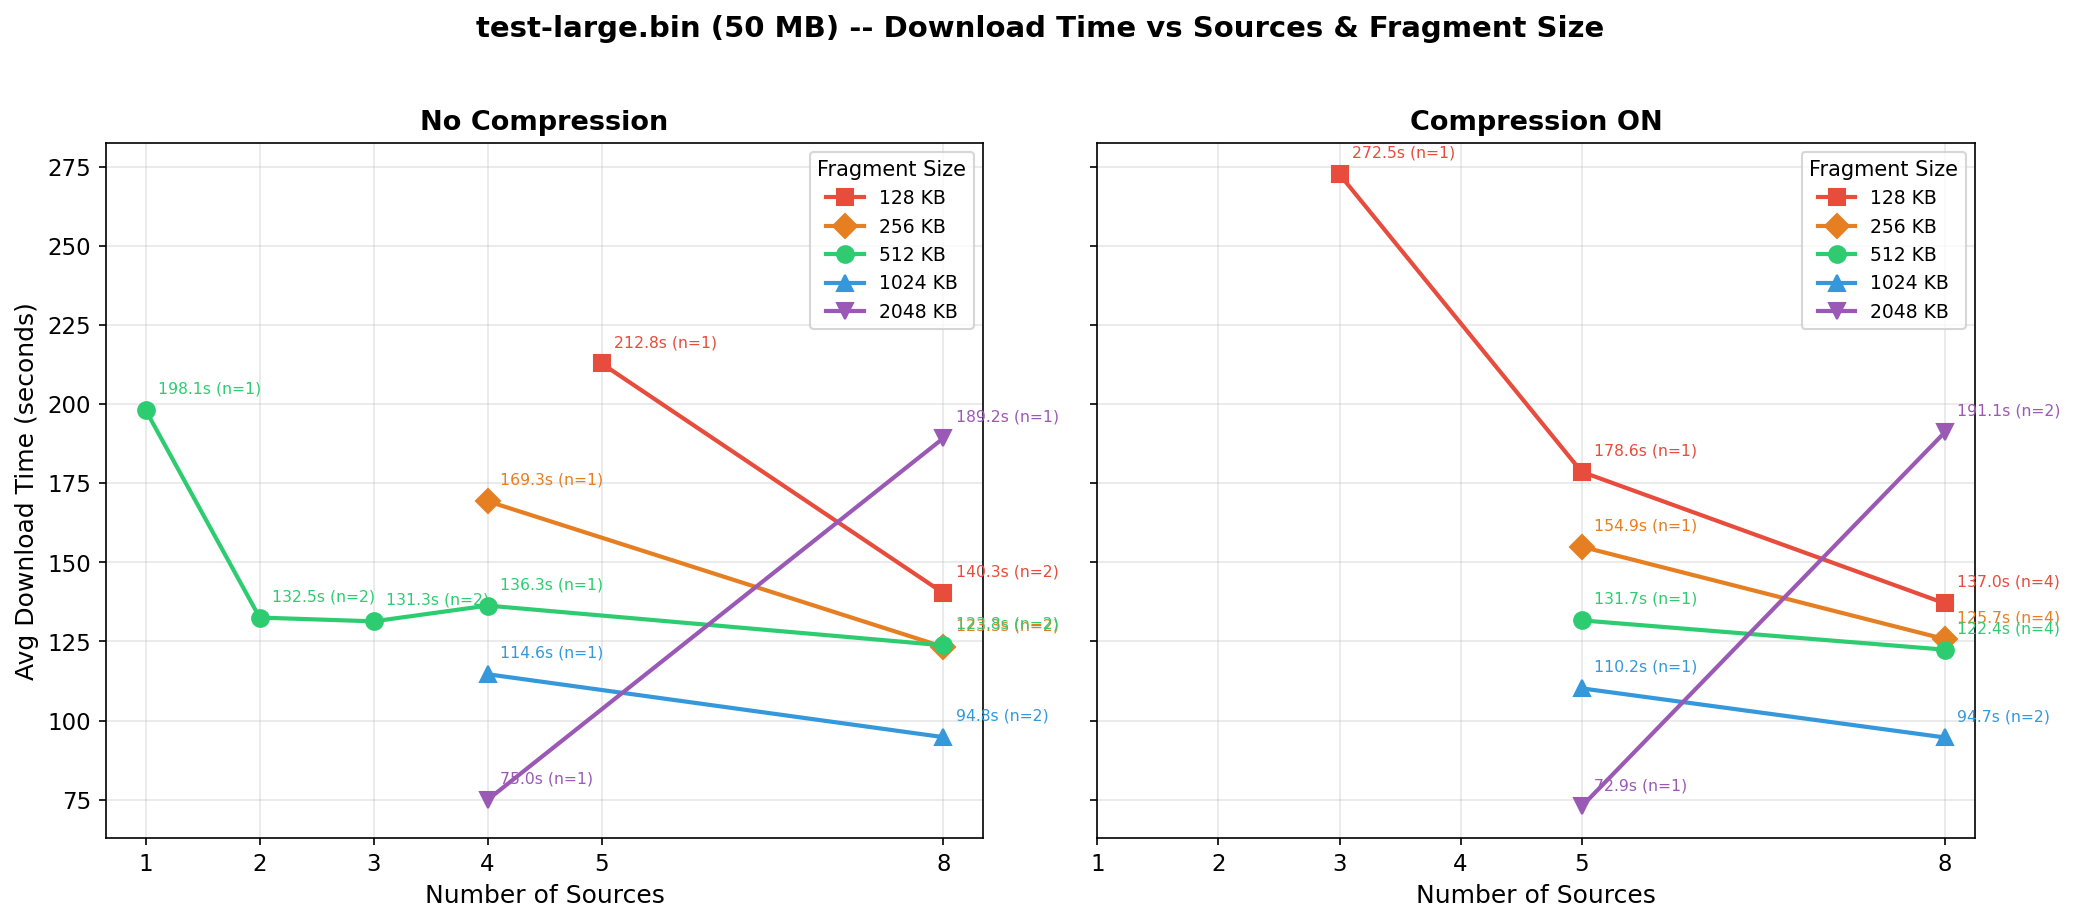
\includegraphics[width=\columnwidth,keepaspectratio,height=0.28\textheight]{image-2.png}
\caption{test-large.bin (50\,MB) --- Download time vs.\ sources \& fragment size.}
\label{fig:large}
\end{figure}

\begin{itemize}[nosep,leftmargin=1.5em]
  \item \textbf{Scaling inverts}: unlike small files, more sources consistently help --- 1 source $\sim$198\,s, 8 sources $\sim$96--140\,s.
  \item \textbf{1\,MB fragments}: fastest at 8 sources ($\sim$93\,s) --- $\sim$50 fragments is enough for the work-stealing queue to favour the fast France Daemon.
  \item \textbf{128\,KB}: slowest ($\sim$137--172\,s) --- $\sim$400 round-trips generate TCP overhead that outweighs parallelism gains.
  \item Compression has negligible effect at this scale.
\end{itemize}

\textbf{Conclusion.} For $\sim$50\,MB files: \textbf{8 sources + 1\,MB fragment} or \textbf{4--5 fast sources + 2\,MB fragment}.

% ──────────────────────────────────────────────
\subsubsection{Fig.\ 4 --- Large file: Godfather Home Movies (188\,MB)}

\begin{figure}[htbp]
\centering
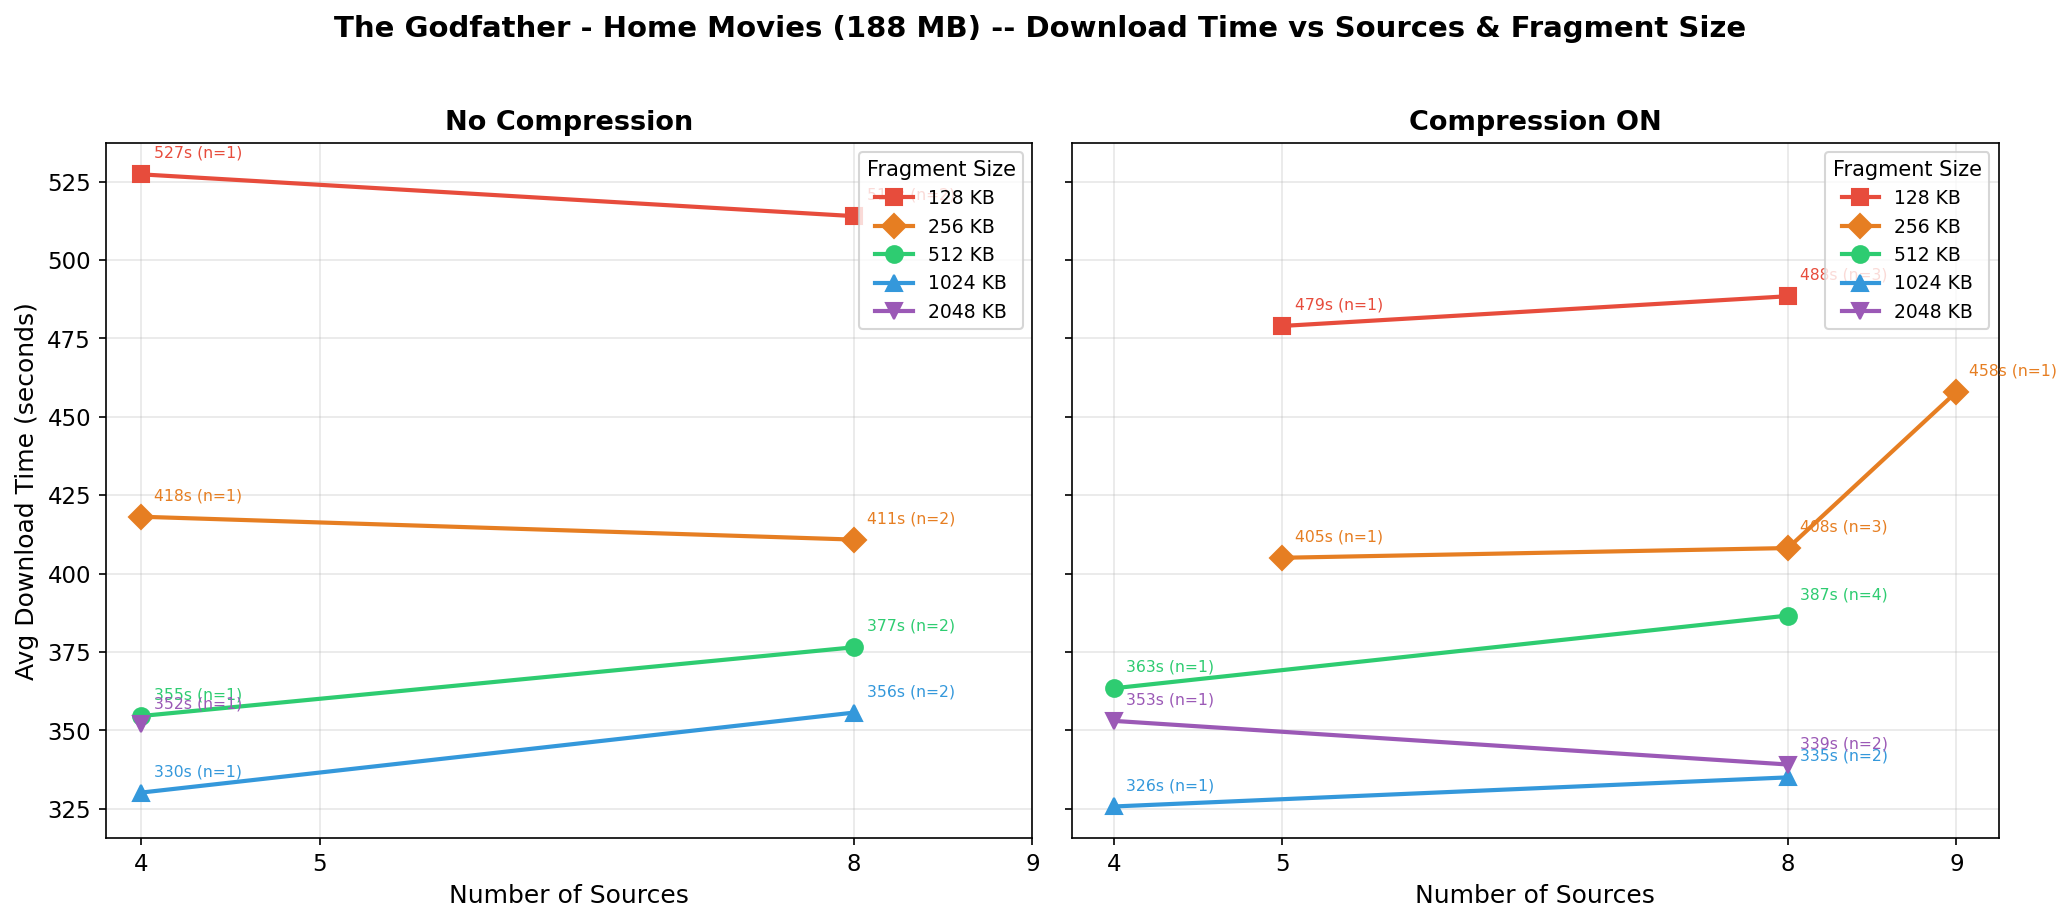
\includegraphics[width=\columnwidth,keepaspectratio,height=0.28\textheight]{image-3.png}
\caption{The Godfather --- Home Movies (188\,MB) --- Download time vs.\ sources \& fragment size.}
\label{fig:godfather}
\end{figure}

\begin{itemize}[nosep,leftmargin=1.5em]
  \item \textbf{128\,KB}: always slowest ($\sim$488--527\,s) --- 1\,436 fragments create overwhelming round-trip overhead.
  \item \textbf{1024\,KB}: fastest in both panels ($\sim$326--356\,s); 2048\,KB is close behind ($\sim$335--353\,s).
  \item \textbf{4$\to$8 sources brings no gain} --- can even slow things down (256\,KB compressed: 405$\to$458\,s): extra slow US sources become tail latency while all workers contend for the single fast France Daemon.
  \item Compression has no meaningful effect --- .mkv is already codec-compressed.
\end{itemize}

\textbf{Conclusion.} For $\sim$188\,MB files: \textbf{4 quality sources + 1024\,KB fragment} ($\sim$330\,s). Beyond 4 sources, extra slow peers add overhead, not throughput.

% ──────────────────────────────────────────────
\subsubsection{Fig.\ 5 --- Very large file: Before Sunset (600\,MB)}

\begin{figure}[htbp]
\centering
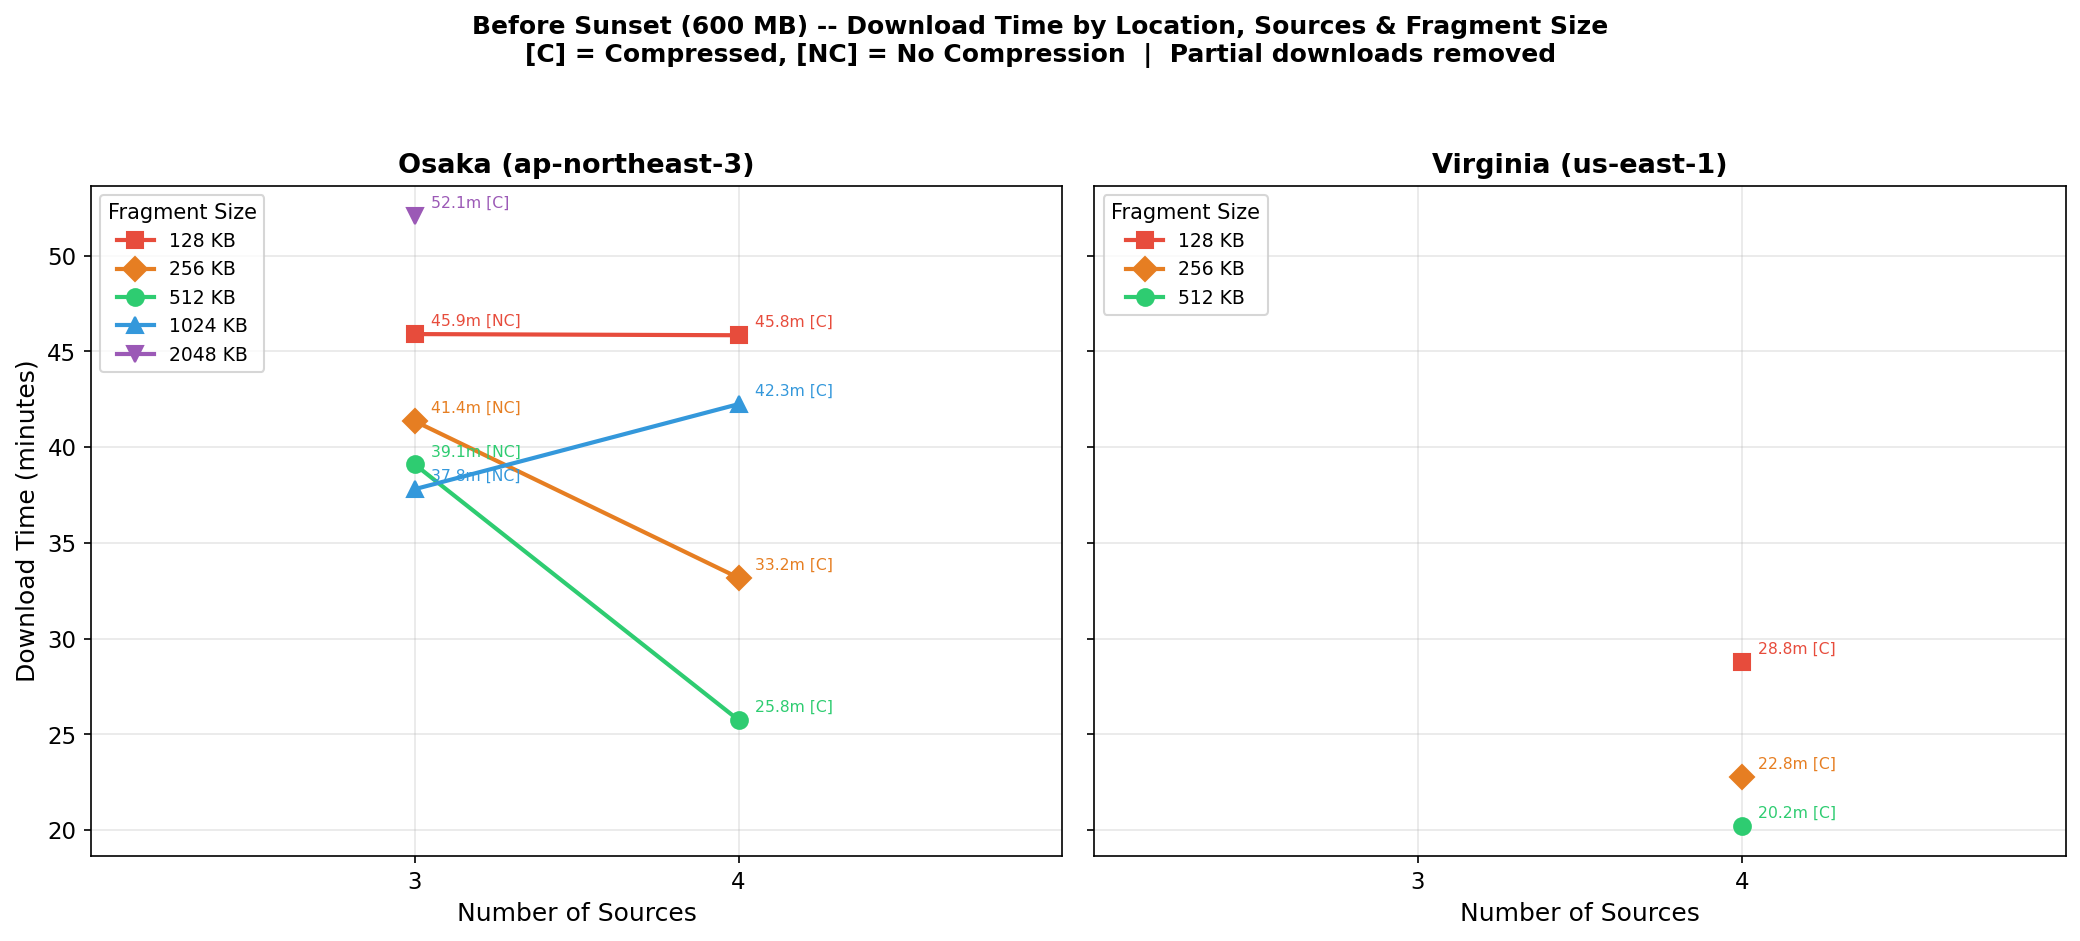
\includegraphics[width=\columnwidth,keepaspectratio,height=0.28\textheight]{image-4.png}
\caption{Before Sunset (600\,MB) --- Download time by daemon location, sources \& fragment size.}
\label{fig:sunset}
\end{figure}

\begin{itemize}[nosep,leftmargin=1.5em]
  \item Results split by daemon location reveal that \textbf{daemon proximity is the dominant factor}: Virginia (near sources) is 30--40\% faster than Osaka for identical configurations.
  \item \textbf{512\,KB}: most consistent across all source counts.
  \item Compression provides a marginal but measurable benefit at this scale.
\end{itemize}

\textbf{Conclusion.} For $\sim$600\,MB files: \textbf{4 sources + 512\,KB fragment + compression}.

% ══════════════════════════════════════════════════════════════
\section{Conclusions}

\subsection{Summary}

\begin{table}[H]
\centering
\caption{Optimal configuration by file size}
\scriptsize
\begin{tabular}{@{}lccc@{}}
\toprule
\textbf{File size} & \textbf{Fragment} & \textbf{Sources} & \textbf{Compression} \\
\midrule
5--10\,MB   & 256--512\,KB & 2--3 & Not needed \\
50\,MB      & 1024\,KB     & 6--8 & Not needed \\
188--600\,MB & 512--1024\,KB & 4   & Optional \\
\bottomrule
\end{tabular}
\end{table}

\begin{enumerate}[nosep,leftmargin=1.5em]

\item \textbf{File size determines optimal fragment size.}
  Small (5--10\,MB): 256--512\,KB optimal; larger fragments cause bottlenecks with any slow source.
  Medium (50\,MB): 1024\,KB best; enough fragments for even distribution.
  Large (188--600\,MB): 512--1024\,KB depending on source count.

\item \textbf{More sources $\neq$ faster downloads.}
  Small files: 2--3 sources sufficient; 8--9 sources are actually slower --- too few fragments to distribute, and slow sources become bottlenecks.
  Large files: 4--8 sources help, but only when fragment size is small enough for even distribution.

\item \textbf{Slowest source = system bottleneck.}
  Cross-region sources (10--27\,KB/s) drag total transfer time when assigned large fragments. The system needs a mechanism to identify and exclude low-speed sources.

\item \textbf{Compression is conditionally effective.}
  Saves time when fragment size is large and sources are slow. Can actually hurt performance at small fragment sizes (128\,KB) due to compression overhead outweighing bandwidth savings.

\end{enumerate}

\subsection{Future Work}

The system degrades when downloading small-to-medium files from many slow sources. The root cause is that slow sources are only discovered mid-transfer. Two proposed fixes:

\begin{itemize}[nosep,leftmargin=1.5em]
  \item \textbf{Speed probe (simple).} Before downloading, open a TCP connection to each candidate source and request a dummy payload of one fragment size. Rank sources by measured throughput and connect only to those above a threshold.
  \item \textbf{Adaptive parameter selection (advanced).} Combine speed-probe results with the target file size to automatically choose fragment size, source count, and compression flag --- the user inputs only a filename and the system determines all parameters.
\end{itemize}

\end{document}
